
a) Den givne formel er skrevet og løst på tableau form:

\begin{figure}[H]
    \centering
    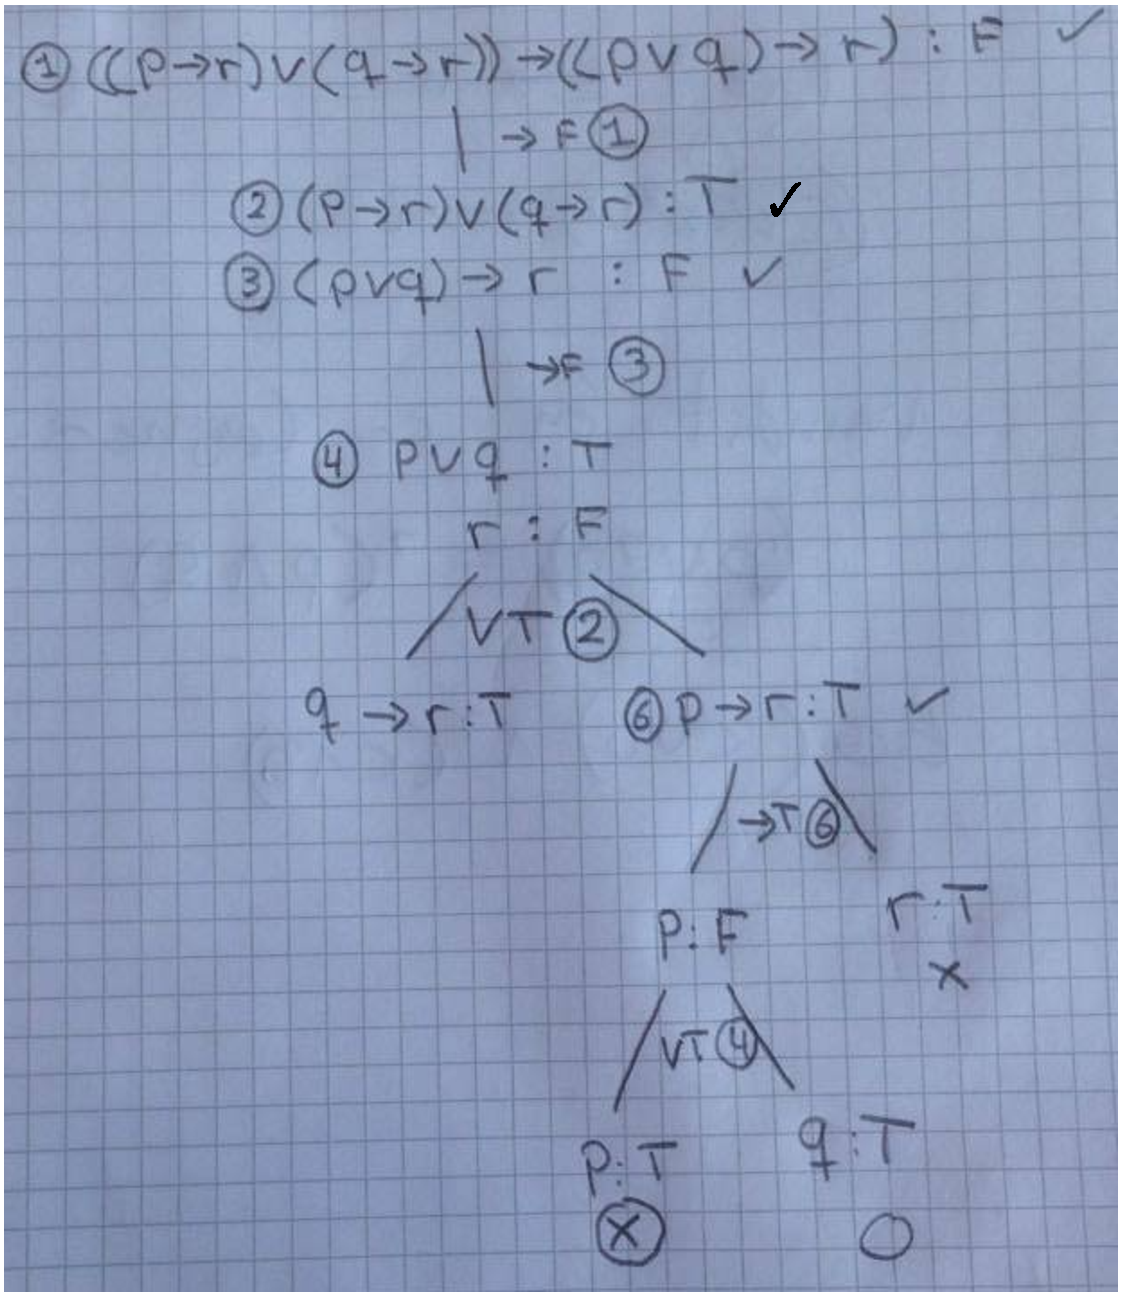
\includegraphics[height=13 cm]{OpgA/tableauAa2.pdf}
    \label{fig:Aa}
\end{figure}

Da en gren fandtes mættet og åben, er formlen opfyldelig med sandhedstildelingen
\begin{equation*}
    r:\text{F},\: p:\text{F}, \: q: \text{T}
\end{equation*}

Man kan vha. en sandhedstabel vise, at også sandhedstildelingen $p:\text{T},\: q:\text{F}, \: r: \text{F}$ er en løsning. Opgaveformuleringen spurgte dog specifikt om tableau-metoden, og bad os om ikke at fortsætte, når vi fandt blot en enkel åben mættet gren.